\documentclass[12pt]{article}

\usepackage[margin=1in]{geometry}
\usepackage{amsmath, amssymb}
\usepackage{enumitem}
\usepackage{booktabs}
\usepackage{graphicx}
\usepackage{float}
\usepackage{longtable}
\usepackage{parskip}
\usepackage{interval}
\usepackage{xcolor}
\usepackage{courier}
\usepackage{setspace}
\intervalconfig {soft open fences}
\setlength{\parindent}{0pt}

% Colorful hyperlinks within document
\usepackage[colorlinks, citecolor={blue}]{hyperref}

% Verbatim display of R or other code
\usepackage{verbatim, listings}

% Formatting for bibliography
\usepackage{natbib}
%\setcitestyle{numbers}
%\emergencystretch=1em

% More options with captions
\usepackage[format=plain,
labelfont={bf,it},
textfont=it]{caption}

% Figure placement obeys instructions
\usepackage{float}

% EXAMPLE FIGURE INCLUSION
% \begin{figure}[H]
% \centering
% \includegraphics[width=.7\linewidth]{figures/hist\_y0}
% \end{figure}

% EXAMPLE CITATIONS
% \citep{rodgers2002alzheimer}
% \citet{holbrook2020anterolateral}

% DOUBLE SPACING
\doublespacing

\title{A multivariate longitudinal model with subject-varying effects for the physical and mental progression of Alzheimer's Disease}
\author{Jesse W.~Birchfield, Robert E. Weiss, and Andrew J. Holbrook}
	
\begin{document}

\maketitle

\pagebreak
\section{Introduction}

Symptoms of Alzheimer's Disease (AD) include both physical and mental decline. Physically, by the prevailing theory \citep{jack2010hypothetical}, amyloid plaques and neurofibrillary tangles progressively destroy the brain's neurons, beginning in the entorhinal cortex (ERC) and then spreading into the hippocampus and elsewhere \citep{holbrook2020anterolateral}. Mentally, subjects begin having difficulty with short-term memory and word recall, and then progressively lose other cognitive and motor abilities \citep{rodgers2002alzheimer}. In principle, the mind may be explicable in terms of the nervous system. In practice, it is not, and may never be. For the description of ``objective" biological processes of the brain on one hand, and the description of ``subjective" experiences and behaviors on the other, we have concepts, tools, and measurements that are not only different but incommensurable. A full account of the progression of AD, then, should include both kinds of description. 

Whereas our previous work had the practical aim of improving cortical thickness estimates and enabling earlier detection, the present work is more purely exploratory. We investigate how the effects of the disease co-evolve over time, in relation to the covariates of age, sex, and diagnostic group (disease stage). Using a dataset from the Alzheimer's Diseases Neuroimaging Initiative (ADNI), the ADNI-1 study \citep{mueller2005ways, jack2008alzheimer, petersen2010alzheimer}, we build a multivariate longitudinal model that includes both physical and mental outcomes for each subject at each timepoint. As a physical outcome, we use the thickness of the entorhinal cortex, as estimated by one or more imaging techniques. As a mental outcome, we use the measure taken by ADNI, performance on the Mini Mental State Examination (MMSE) \citep{tombaugh1992mini}. Our model features hierarchical structure, as varying slopes and intercepts for each subject and outcome (we prefer this term to ``random effects"), with the means and full unstructured covariance matrix of these effects as hyperparameters. This construction enables maximal information sharing across outcomes and subjects, and it allows inference the mean and variance of any of the varying parameters, and the covariance between any subset of them. We discuss all of this in more depth below.

Immediately, we face an array of challenges. First is the challenge of imaging. For brain measurements, we start with magnetic resonance images (MRI), then use different computational ``pipelines" to assemble them into a three-dimensional images, ``segment" them into distinct tissue types, ``label" them as different structures, then estimate their volume and thickness \citep{tustison2021antsx}. Although sophisticated, these imaging pipelines are still subject to measurement error. Between pipelines, we see different estimates from the same scan. Within the same pipeline, between scans of the same individual, we see variation beyond that which can explained biologically. The magnitude of measurement error is large enough that it threatens to drown out the subtle effects we hope to detect statistically. And there is no ground truth or gold standard by which to measure the accuracy of these pipelines; we are limited to metrics of internal consistency and predictive power. See our previous work \citep{birchfield2022synthesizing} for an attempt to address this issue.

Second is the challenge of psychometrics. Next to the technological marvels of MRI machines and imaging algorithms, a brief questionnaire like the MMSE is very simple and cheap to administer and score. But it is difficult to determine what, exactly, is the construct being measured, or what real entity a score (or score difference) corresponds to, or how accurate the instrument is as an estimator of that construct, or how accurate is an individual instance of measurement. The problem of no ground truth is more pronounced than for the task of imaging, because here it is hard to say even in theory what form ground truth would take. These are interesting and important issues, but beyond the scope of this research. 

Third is the challenge of combining the two measures in a longitudinal model. Brain decay, for a single individual, does not occur uniformly throughout the organ, or at a steady tempo \citep{holbrook2020anterolateral}. Across individuals, the spatial and temporal decay patterns vary as well, possibly dependent on factors both measured and unmeasured. We should not expect a simple or consistent pattern of mental decline, either. Even the correlation between physical and mental symptoms is not straightforward. For example, subjects may silently experience several years of brain damage before manifesting any cognitive impairment, and subjects with similar levels of brain damage may perform very differently on cognitive assessments \citep{rodgers2002alzheimer}. We propose a model flexible enough to capture this complexity and heterogeneity across outcomes, across time, and across subjects. 

Our different outcomes also have very different numerical properties. Consistent with the hypothesis that they are generated as the true value plus a possible constant bias plus a random measurement error, ERC thickness estimates are positive real numbers with a ``smooth", unimodal, symmetric distribution. A Gaussian fits easily. As questionnaire scores, however, MMSE values are integers, thus discrete and ``coarse"; bounded, on a scale of 0 to 30; and with a very pronounced mode at the right boundary (30) and a long left tail. A Gaussian could hardly do worse. Still, the multivariate normal model has such clear advantages that we would like to adapt our data to the model, rather than the other way around. We propose a transformation of the MMSE data to make this possible. 

We don't just specify a single model \textit{a priori}. After some experimentation with model structure, we build eight models of the chosen class, with different configurations of ERC pipeline and MMSE transformation. We compare their predictive power with Bayesian 5-fold cross-validation. Since the models have different numbers of observations and outcomes on different scales, we use a novel combination of techniques to construct a metric comparable across all the models. 

{\color{teal} [Literature review here]}

{\color{teal} [Interpretation: what do we learn from the model?]}

\pagebreak
\section{Data}

Our data comes from the Alzheimer's Disease Neuroimaging Initiative (Jack Jr et al., 2008; Petersen et al., 2010; Mueller et al., 2005), a public-private partnership sponsored in part by the National Institute on Aging (NIA). Beginning in October 2004, the three-year longitudinal ADNI-1 study followed a cohort of North American patients comprising 200 elderly controls, 400 with mild cognitive impairment (MCI), and 200 with diagnosed Alzheimer's Disease (AD). At each visit, researchers conducted cognitive assessments and structural MRI scans. Our analysis uses data from 663 of the 800 patients tabulated and made publicly available in Tustison et al. (2019), with a total of 2449 visits. We simply omit those visits that had missing MMSE scores.

\begin{figure}[H]
\centering
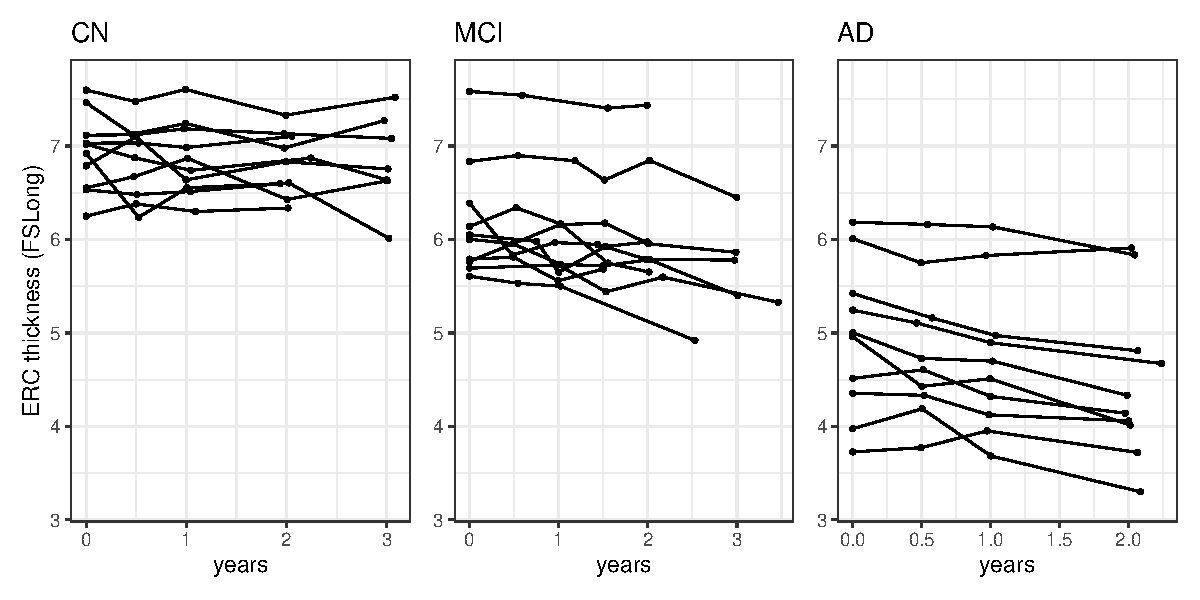
\includegraphics[width=\linewidth]{figures/profiles_by_diagnosis}
\caption{From those who had at least 4 visits (or at least 3 for the AD group), we select 10 subjects at random from each diagnostic group and plotted their ERC thickness over time, as measured by the FreeSurfer pipeline. Comparing MCI to CN, we see more variance in initial thickness, slightly lower average initial thickness, and slightly more downward of a trend overall. Comparing AD to MCI, we see even more variance in initial thickness, much lower average initial thickness, and a more noticeable downward trend overall.} 
\end{figure}

We analyze output from two ERC thickness pipelines. FreeSurfer (FS) \citep{fischl2012freesurfer} and Advanced Normalization Tools (ANTs) \citep{avants2009advanced} use different geometrical constructs to stand in for cortical thickness. FreeSurfer is mesh based, using polygonal meshes representing the gray/white matter surfaces and outer cortical surfaces. We use the version of FreeSurfer optimized for longitudinal measurements of the same subject, hereafter FSLong. ANTs is volumetric, using diffeomorphic mappings, which are smooth manifolds. We use the version of ANTs optimized for repeated measurements of the same subject, called the ``single subject template", hereafter ANTsSST. 

\begin{figure}[H]
\centering
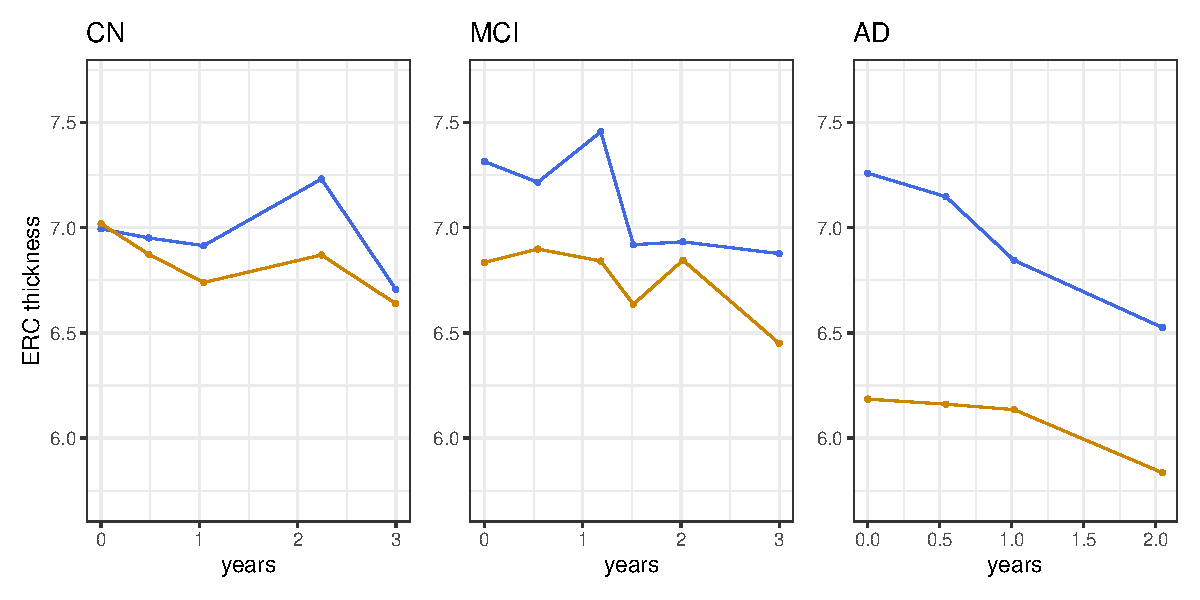
\includegraphics[width=\linewidth]{figures/profiles_by_pipeline}
\caption{From each diagnostic group, we choose one subject at random and plot the longitudinal profile of ERC thickness, as measured by FSLong (orange) and ANTsSST (blue). This small sample suggests that ANTsSST tends to give consistently larger estimates. The deviations from parallel suggest uncorrelated measurement errors between the two pipelines. We explore the differences in more depth in \citep{birchfield2022synthesizing} and in the Results section of this paper.} 
\end{figure}

The MMSE is a screening test for cognitive impairment. It has 10 questions, takes 5 to 10 minutes to administer, and covers space and time orientation, naming familiar objects, repeating back a phrase, recalling a previous question, manipulating letters and/or numbers, and following instructions. Out of 30 possible points, a score of 24 or more indicates normal cognition, 19-23 indicates mild cognitive impairment, and 18 or below indicates moderate or severe impairment. While it can help differentiate different types of dementia, the test itself is not sufficient for diagnosis.

\begin{figure}[H]
\centering
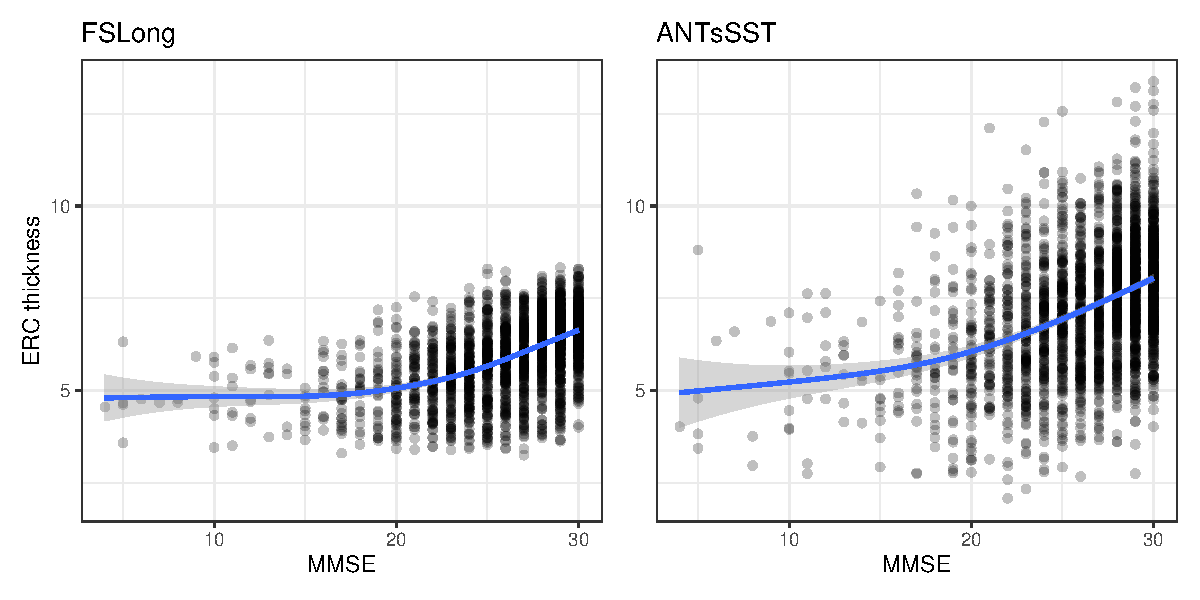
\includegraphics[width=\linewidth]{figures/erc_mmse_scatterplot}
\caption{Above are ERC thicknesses, as measured by FSLong (left) and ANTsSST (right) compared to MMSE score, for all observations without respect to individual or time. Both pipelines show a weak positive correlation with much unexplained variation. ANTsSST estimates a greater range of ERC thicknesses.} 
\end{figure}

\pagebreak
\section{Methods}

\subsection{Rationale for model design}

In our full models, for each brain scan, we include the FSLong and ANTsSST measurements of ERC thickness as a bivariate outcome. Good statistical practice is to incorporate as much relevant information as possible in the model. Our previous work suggests that FSLong and ANTsSST have complementary advantages for estimating ERC thickness. For example, it appears that FS overall more consistent, but is also more likely to have large outliers. Since they use very different algorithms, their errors are likely uncorrelated, and if so, an estimator derived from both of them will have smaller variance. A more unusual design choice is to include MMSE as a third joint outcome, rather than a covariate. In our previous work, we specified ERC as a predictor of MMSE. However, there is an asymmetry between the interpretation of explanatory and outcomes variables in all but the simplest statistical models, especially when other covariates are present. By specifying ERC and MMSE as joint outcomes, we avoid making any assumptions about dependence. Instead, we look at covariance over time. In our models, the only time-varying covariate is time itself, making interpretation more straightforward. See \citet{weiss2005modeling} for a longer discussion of the advantages of multivariate outcomes in longitudinal models.

As discussed earlier, the Gaussian distribution does not fit MMSE scores. A natural choice for the joint distribution would be a bivariate normal for ERC thickness measurements plus, say, a zero-inflated negative binomial for MMSE scores (2VN+ZINB). Still, the multivariate normal distribution has two huge advantages. First, it can share information across outcomes via the error covariance matrix. That is, the observed values of outcome $y_1$ inform the estimation of the parameters explaining $y_2$, and can help impute a missing value of $y_2$. With a 2VN+ZINB model, information sharing only occurs through the covariance of the subject-varying effects. For this data at least, model-fitting and cross-validation statistics reveal that a 2VN+ZINB model does no better at explaining or predicting ERC thickness than a model for ERC thickness alone, no better for MMSE than a model for MMSE alone, and worse overall than even a naive MVN model. Second, by a property of the multivariate normal distribution, we can analytically specify the conditional mean and variance of any subset of the outcome vector $\boldsymbol{Y}$ in terms of the remaining elements. If we let 
$$ \boldsymbol{Y} = \boldsymbol{ \begin{bmatrix} Y_a \\ Y_b \end{bmatrix} } \sim
N \boldsymbol{ \left(
\begin{bmatrix} \mu_{a} \\ \mu_{b} \end{bmatrix},
\begin{bmatrix} V_{aa} & V_{ab} \\ V_{ba} & V_{bb} \end{bmatrix}
\right) }, $$
then it follows that
$$ \boldsymbol{ Y_b | \{ Y_a = y_a \} \sim 
N( \mu_b + V_{ba} V^{-1}_{aa}(y_a - \mu_a), V_{bb} - V_{ba} V^{-1}_{aa} V_{ab} ) }.$$
See \citet{seber2012linear} for a proof. {\color{teal} [I have improved on the exposition of their proof; should I include it as an appendix?].} With this formula, we can specify ERC thickness in terms of MMSE and the covariates, or MMSE in terms of ERC thickness and the covariates, in a symmetric fashion. It will prove useful for inference and indispensable for model comparison. 

\pagebreak
\subsection{MMSE transformation}

The 2449 observations of MMSE look like this. Clearly, they do not satisfy the normality assumption, and a multivariate normal model will give poor results. A Gaussian distribution describes a continuous quantity, not a discrete one. MMSE score is literally a count variable--the number of questions answered correctly on the questionnaire. 

\begin{figure}[H]
\centering
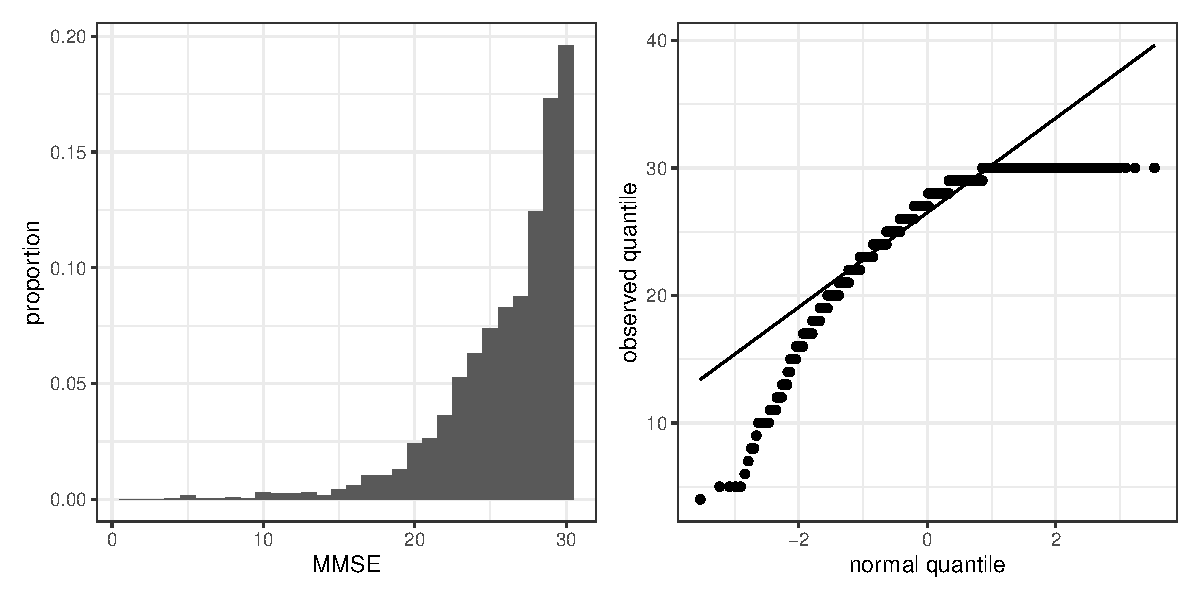
\includegraphics[width=\linewidth]{figures/mmse_before}
\caption{Left: a relative frequency histogram of raw MMSE score for all subjects. It is discrete (integer-valued), bounded (0 to 30), and left-skewed, with a strong mode at the right endpoint. All of these features make it difficult to model with a Gaussian distribution. Right: a normal qq-plot for MMSE. It shows a very poor fit.}
\end{figure}

But since the MMSE's objective is to somehow quantify cognitive capacity, which can reasonably be thought of as continuous, we can treat MMSE score as a ``coarse" or rounded measurement of a continuous latent variable. Our first transformation is to consider ``MMSE loss"--questions missed--rather than MMSE, by subtracting the raw value from 30. So a score of 30 becomes 0, a score of 29 becomes 1, and so on. We also imagine a kind of threshold, where cognitive decline has to reach a certain point before the subject would miss another question, so the MMSE loss represents a rounding \textit{down} of the latent quantity. This justifies the step of adding $0.5$ to each value. So define $y = 30 - MMSE + 0.5$. Our next step is much easier with a single-parameter probability distribution, and this looks like a histogram of a sample from some Exponential distribution. (The half-normal is another candidate, but we find that it gives poorer results on this data.) We assume $F(y) = 1 - e^{-\lambda y}$. The maximum likelihood estimate of $\lambda$ is the maximum value of the polynomial $\Pi_{i=1}^{n}\left[ e^{-\lambda y_i} - e^{-\lambda (y_i + 1)} \right]$, which R easily computes as $\hat{\lambda} = 0.236$. The probability integral transform states that if random variable $W$ has continuous monotonic CDF $F$, then random variable $F(W)$ has a $Unif(0,1)$ distribution. Conversely, if $U \sim Unif(0,1)$, and $G$ is the continuous monotonic CDF of random variable $X$, then random variable $G^{-1}(U)$ has the same distribution as $X$. Letting $F$ in the theorem be the exponential CDF with parameter $\hat{\lambda}$, and letting $G$ be the standard normal CDF $\Phi$, the transformation $\Phi^{-1}(F(Y))$ will have standard normal distribution, at least to the extent that $F$ describes the distribution of $Y$. 

\begin{figure}[H]
\centering
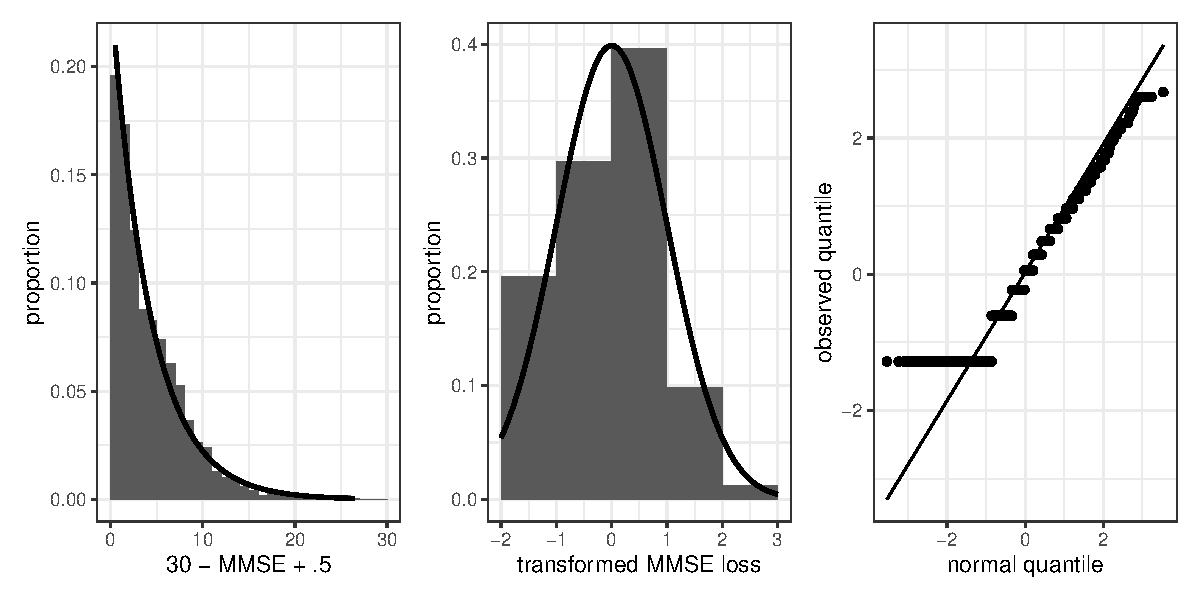
\includegraphics[width=\linewidth]{figures/mmse_after}
\caption{Left: Histogram of MMSE loss, defined as $30 - MMSE + .5$, overlaid with an Expo(.236) density, the best-fitting Exponential model by maximum likelihood. The histogram looks like a plausible sample from this density. Center: a histogram of MMSE transformed according to $h(y) = \Phi^{-1}(1 - e^{-.236(30-y+.5)})$, overlaid with a N(0,1) density. While not a perfect fit, it is a substantial improvement on the original. Right: a normal qq-plot of transformed MMSE loss. The main departure from normality occurs because of the high number of perfect MMSE scores.}
\end{figure}

It is true that this technique will give $Y$ a \textit{marginally} normal distribution, whereas the assumption of the multivariate normal regression model is that $Y$ is \textit{conditionally} normal given the predictors. But this is does not make much of a difference in practice. If $Y|X \sim N(X\beta, \sigma_{Y}^{2})$, and $X \sim N(\mu_X, \sigma_{X}^{2})$, then $Y \sim N(\mu_X, \sigma_{X}^{2} + \sigma_{Y}^{2})$; it is still normal. If $X$ is binary or discrete, then $Y$ is a mixture of normals; when the differences between the means of the mixture components are small compared to the overall variance, the mixture distribution is empirically not much different from a true normal distribution with the same mean and variance. 

\pagebreak
\subsection{Model specification}

Here we describe the model in prose, and afterward we formally specify it in symbols. For each subject, and at each timepoint, we have a bivariate or trivariate outcome, consisting of (i) ERC, as estimated by FSLong, ANTsSST, the arithmetic mean of the two, or both, and (ii) MMSE loss, either untransformed or transformed. We model these as bivariate or trivariate normal, where the mean is a linear function of predictors described below, and the error covariance matrix is unstructured, to be estimated from the data. Predictors are age at baseline centered by subtracting the mean age at baseline across all 663 subjects, a gender indicator, and time of visit in years since baseline. For each outcome, we have a separate set of coefficients. The coefficients for age and gender are ``fixed", in the sense that they do not vary by subject and do not have hyperparameters. The intercepts and slopes of the outcomes \textit{do} vary by subject, and we consider them as draws from an underlying multivariate normal distribution with a common mean and an unstructured covariance matrix. This hierarchical structure allows for information sharing across outcomes, across timepoints, and across subjects. We do not add any additional covariance across timepoints other than that induced by the slopes. Finally, for each diagnostic group--CN, MCI, AD--we fit a completely separate set of coefficients and hyperparameters, so that we are effectively performing three separate regressions. 

Formally, let $i$ index subjects, $i=1,...,N$. For our data, $N = 663$. Let $j$ index timepoints, $j = 1, ..., J_i$. For our data, $J_i$ is between 2 and 6 for all $i$. Let $k$ index outcomes, $k=1,...,K$. For models 1-3 and 4-6, $K = 2.$ For models 4 and 8, $K = 3$. Let $\ell$ index groups, $\ell=1,...,L$. For our data, $\ell=1,2,3$ for CN, MCI, AD respectively. Let $m$ index covariates or coefficients. So we have five sets of indices $i,j,k,\ell,m$, not all of which are relevant for any given quantity. To avoid confusion, we use dots as placeholders for irrelevant indices, so that $x_{7...2}$ is covariate $m=2$ for subject $i=7$, which is the same for all timepoints $j$ and outcomes $k$ and has group $\ell$ determined by $i$. 

Let $\boldsymbol{y_{ij.\ell}}$ be the $K$-vector of observation $ij$, where subject $i$ is in group $\ell$. Let $\boldsymbol{\epsilon_{ij.\ell}}$ be the $K$-vector of errors for observation $ij$, for $i$ in group $\ell$. Both for computation and for interpretability, we factor all covariance matrices into a diagonal matrix of standard deviations and a matrix of correlations, e.g. $\boldsymbol{C=SRS'}$, and we write the standard deviations as a vector. Then, when specifying multivariate normal distributions, we use the notation $N$(mean, sd vector, correlation matrix). Let $\boldsymbol{\sigma_{...\ell}}$ be the $K$-vector of standard deviations for the error vectors $\boldsymbol{\epsilon_{ij.\ell}}$, and let $\boldsymbol{R_{...\ell}}$ be the $K \times K$ correlation matrix.

Let $x_{i...1}$ be baseline age in years, mean-centered, for subject $i$. Let $x_{i...2}$ be the indicator that subject $i$ is male, for subject $i$. Let $\boldsymbol{x_{ij..}'} = \begin{bmatrix}x_{ij..1} & ... & x_{ij..M}\end{bmatrix}.$ Generally, we use $\alpha$ to denote subject-invariant effects and $\beta$ to represent subject-varying effects. Let $\boldsymbol{\alpha_{..k\ell}'}$ be the 2-vector of coefficients for each $\boldsymbol{x_{ij..}'}$ outcome $k$, group $\ell$. Let $t_{ij...}$ be time in years since baseline for subject $i$, timepoint $j$. Let $\boldsymbol{z_{ij...}'} = \begin{bmatrix} 1 & t_{ij..} \end{bmatrix}$. Let $\boldsymbol{\beta_{i.k\ell}}$ be the 2-vector of subject-varying intercept and slope for subject $i$, outcome $k$, group $\ell$. Let $\boldsymbol{\beta_{i..\ell}}$ be the concatenated $2K$-vector $\begin{bmatrix} \boldsymbol{\beta_{i.1\ell}'} & ... & \boldsymbol{\beta_{i.K\ell}'} \end{bmatrix}'$. Let  $\boldsymbol{\mu_{...\ell}}$ be the $2K$-vector of means for the vectors $\boldsymbol{\beta_{i..\ell}}$, let $\boldsymbol{\tau_{...\ell}}$ be the $2K$-vector of standard deviations, and let $\boldsymbol{\Omega_{...\ell}}$ be the $2K \times 2K$ correlation matrix. 

This complexity of notation pays off, because it allows us to express the model quite compactly, as
$$
\boldsymbol{y_{ij.\ell}} = 
\begin{bmatrix}
	\boldsymbol{x_{ij..}'\alpha_{..1\ell} + z_{ij..}'\beta_{i.1\ell}} + \epsilon_{ij1\ell} \\
	\boldsymbol{x_{ij..}'\alpha_{..2\ell} + z_{ij..}'\beta_{i.2\ell}} + \epsilon_{ij2\ell} \\
	\boldsymbol{x_{ij..}'\alpha_{..3\ell} + z_{ij..}'\beta_{i.3\ell}} + \epsilon_{ij3\ell}	
\end{bmatrix}
$$
$$
\boldsymbol{\beta_{i..\ell}} \mid \ \boldsymbol{\mu_{...\ell}}, \boldsymbol{\tau_{...\ell}}, \boldsymbol{\Omega_{...\ell}}
\sim
N_4 \left(\boldsymbol{\mu_{...\ell}}, \boldsymbol{\tau_{...\ell}}, \boldsymbol{\Omega_{...\ell}}\right)  
$$
$$
\boldsymbol{\epsilon_{ij.\ell} \mid \sigma_{...\ell}, R_{...\ell}}
\sim 
N_2 \left(\boldsymbol{0, \sigma_{...\ell}, R_{...\ell}}\right).
$$

We choose our priors to be as uninformative as possible while still allowing decent convergence in posterior sampling. We keep them identical across models and groups, and virtually identical across outcomes and coefficients. All prior distributions are independent of each other unless otherwise stated. Error sd's have prior $Expo(1)$, parameterized by rate. All $\alpha$ parameters have prior $N(0,2)$. For ERC outcomes, means of subject-specific intercepts have prior $N(7,3)$ and sd's have $Expo(1)$, while means of subject-specific slopes have prior $N(0,1)$ and sd's have $Expo(5)$. For MMSE outcomes, means of subject-specific intercepts have prior $N(0,2)$ and sd's have $Expo(1)$, while means of subject-specific slopes have prior $N(0,2)$ and sd's have $Expo(1)$. Finally, all correlation matrices have prior $LKJCorr(1)$. This is the Lewandowski-Kurowicka-Joe distribution, a single-parameter family of correlation matrices, argued to be superior to the traditional inverse Wishart prior distribution \citep{gelman1995bayesian}. A prior parameter $\eta=1$ indicates neutrality about whether the correlation is positive or negative. 

Our eight candidate models have the same structure, differing only in the  outcome variables, as shown in Table 1:

\begin{table}[H]
\centering
\caption{Candidate models}
\begin{tabular}{|l|l|l|l|}
\toprule
model & $y_1$ & $y_2$ & $y_3$\\
\midrule
1 & untransformed MMSE & FSLong & \\
2 & untransformed MMSE & ANTsSST & \\
3 & untransformed MMSE & ECTavg & \\
4 & untransformed MMSE & FSLong & ANTsSST \\
1 & transformed MMSE & FSLong & \\
2 & transformed MMSE & ANTsSST & \\
3 & transformed MMSE & ECTavg & \\
4 & transformed MMSE & FSLong & ANTsSST \\
\bottomrule
\end{tabular}
\end{table}

\pagebreak
\subsection{Computation}

We use the R programming language, supplemented by the packages \texttt{pacman} for package management; \texttt{dplyr}, \texttt{glue}, and \texttt{stringr} for data management \citep{dplyr, stringr}; \texttt{pracma} for advanced mathematical operations \citep{pracma}; and \texttt{ggplot2} and \texttt{patchwork} for graphics \citep{ggplot2, patchwork}. To specify and fit the model, we use Stan, an open-source Bayesian software application \citep{carpenter2017stan}, interfacing with R through the \texttt{cmdstanr} and \texttt{rstan} packages \citep{rstan}. For additional model diagnostics, we recommend the \texttt{loo} package \citep{vehtari2017practical, loo}, and for visualization and interactive exploration of model convergence, the \texttt{shinystan} package \citep{muth2018user}. We include our model scripts as an appendix, and the Stan file and all R scripts and regression results at \url{ https://github.com/jwbirchfield/ad\_progression/ }. Stan uses Hamiltonian Monte Carlo, a flavor of Markov Chain Monte Carlo to draw samples--each of which is a complete vector of parameters--from the joint posterior distribution \citep{neal2011mcmc}. An advanced extension of HMC called the No U-Turn Sampler (NUTS) improves sampling efficiency \citep{hoffman2014no}. As the number of MCMC samples increases, the distribution of MCMC samples converges to the actual joint posterior distribution. Fortunately, the marginal distribution of each parameter in the MCMC samples converges to its actual marginal posterior distribution as well. To fit each of the eight models, we run 4 chains in parallel with 6000 iterations each, which we thin by a factor of 3 to get 8000 iterations. Effective sample sizes are all no less than 200, and R-hat statistics are no greater than 1.02 \citep{gelman1995bayesian}. See Appendix A for the Stan code for the model. In the cross-validation stage, for each of the eight models and for each of the 5 folds, we run 4 chains in parallel with 2000 iterations each, which we thin by a factor of 2 to get 4000 iterations. 

\pagebreak
\subsection{Model comparison}

\subsubsection{Preliminaries}

Before we compare the models, we need to find some common reference frame by which to compare them. Since FSLong and ANTsSST are on the same scale, models 1-3 are directly comparable to each other by log-likelihood or information criteria. However, they are not comparable to model 4, because it has a trivariate instead of bivariate outcome. Similarly, models 5-7 are comparable to each other but not to model 8. Furthermore, models 1-4, with untransformed MMSE, are not comparable to models 5-8, with transformed MMSE. 

We demonstrate our technique on model 8, the most complicated case. Ignoring subject and timepoint subscripts for now, the outcome vector has the form $\boldsymbol{z}' = \begin{bmatrix} y_1 & y_2 & z \end{bmatrix}$ (note the distinction between bold type for vector and regular type for scalar), where $y_1$ is FSLong measurement of ERC thickness, $y_2$ is the ANTsSST measurement of ERC thickness, and $z$ is transformed MMSE score. If $y_3$ is untransformed MMSE score, then $z = h(y_3) = \Phi^{-1} (1 - e^{-.236 (30 - y_3 + .5})$. To find the inverse, we solve $z = h(y_3)$ for $y_3$:
$$ \Phi(z) = 1 - e^{-\hat{\lambda} y_3} $$
$$ \Rightarrow e^{-\hat{\lambda} y_3} = 1 - \Phi(z) $$
$$ \Rightarrow -\hat{\lambda} y_3 = \log(1 - \Phi(z)) $$
$$ \Rightarrow y_3 = h^{-1}(z) = -\frac{1}{\lambda} \log (1 - \Phi(z)). $$
Next, take the absolute value of the derivative, denoting the standard normal PDF with $\phi$, to get
$$ \left| \frac{dy_3}{dz} \right| = \frac{\phi(z)}{\hat{\lambda} (1 - \Phi(z))} $$
$$ \Rightarrow \log \left| \frac{dy_3}{dz} \right| = \log(\phi(z)) - \log(\hat{\lambda}) - \log(1 - \Phi(z)) $$
$$ \Rightarrow -\log \left| \frac{dy_3}{dz} \right| = -\log(\phi(z)) + \log(\hat{\lambda}) + \log(1 - \Phi(z)). $$
Let $j(z)$ denote the right-hand side of the last equation above. By change of variables, 
$$ f_Y(y_3)  = \frac{f_z(z)}{\left| \frac{dy_3}{dz} \right|} $$
$$ \Rightarrow \log(f_y(y_3)) = \log(f_z(z)) - \log \left| \frac{dy_3}{dz} \right| $$
$$ \Rightarrow \log(f_y(y_3)) = \log(f_z(z)) + j(z). $$
Of the three outcome variables, we have only transformed $y_3$. Therefore, if $\boldsymbol{y} = \begin{bmatrix} y_1 & y_2 & y_3 \end{bmatrix}$ and $\boldsymbol{z} = \begin{bmatrix} y_1 & y_2 & z   \end{bmatrix}$, and $\boldsymbol{\theta_y}$ and $\boldsymbol{\theta_y}$ represent the total parameter vectors for $\boldsymbol{y}$ and $\boldsymbol{z}$, then the above equation implies that
$$ \log(f_{\boldsymbol{y}}(\boldsymbol{y}; \boldsymbol{\theta_y})) = \log(f_{\boldsymbol{z}}(\boldsymbol{z}; \boldsymbol{\theta_z})) + j(z). $$
Writing the PDFs as log-likelihoods, we have 
$$ \ell(\boldsymbol{\theta_y}; \boldsymbol{y}) = \ell(\boldsymbol{\theta_z}; \boldsymbol{z}) + j(z), $$
and summing over all the observations gives
$$ \underset{ij}{\Sigma} ~ \ell(\boldsymbol{\theta_y}; \boldsymbol{y_{ij}}) = \underset{ij}{\Sigma} ~ \left[ \ell(\boldsymbol{\theta_z}; \boldsymbol{z_{ij}}) + j(z_{ij}) \right]. $$
When we fit model 8, we infer $\boldsymbol{\theta_z}$ and not $\boldsymbol{\theta_y}$, but this technique allows us to calculate $\ell(\boldsymbol{\theta_y}; \boldsymbol{y_{ij}})$ regardless. Conveniently, $j(z_{ij})$ does not depend on $\boldsymbol{\theta_z}$, so we can calculate it ahead of time and add it to the log-likelihood when needed. 

This Jacobian adjustment allows us to compare the log-likelihood of model 8 to that of model 4, which is the corresponding model without the MMSE transformation. But we still need a way to compare it to the bivariate models, which have a different number of observations. To do this, we focus the outcome variable common to all the models: MMSE score. Although it would be simpler to use the unconditional log-likelihood, i.e. 
$$ \underset{ij}{\Sigma} ~ \ell(\boldsymbol{\theta}; y_{ij3}) = \underset{ij}{\Sigma} ~ \log \left(\phi \left( \frac{y_{ij3} - \mu_{i3}}{\sigma_3} \right) \right),$$ 
to do so would ignore the inferred error correlations, a crucial feature of the models. Instead, we use the \emph{conditional} log-likelihood, 
$$ \underset{ij}{\Sigma} ~ \ell(\boldsymbol{\theta}; y_{ij3}) = \underset{ij}{\Sigma} ~ \log \left(\phi \left( \frac{y_{ij3} - \mu_{i3}^{*}}{\sigma_{3}^{*}} \right) \right),$$ 
where $\mu_{i3}^{*}$ and $(\sigma_{3}^{*})^2$ are the conditional mean and variance from the formula in Section 3.1. In summary, we are working with a quantity that is computable and comparable across all 8 models: the Jacobian-adjusted (when necessary), likelihood (or log-likelihood) of observed MMSE score, conditional on the other outcome(s). Instead of repeating this unwieldy phrase, we denote it with $JACL$ or $JAC\ell$ ($L$ for likelihood, $\ell$ for log-likelihood). 

Since we have $S$ MCMC samples from the posterior distribution of the parameter vector, we have $S$ samples of the $JACL$ or $JAC\ell$ for each of the $N$ observed MMSE scores. We can reduce this to a single fit statistic defined in  \citet{vehtari2017practical}, called the expected log predictive density (ELPD), although to be accurate it should be called the log expected predictive density. Arrange the values in an $S \times N$ matrix, so that element $(s,n)$ is the $s^{th}$ sample of the $JACL$ (likelihood, not log-likelihood) of the $n^{th}$ MMSE score. Take the products of each row (the total likelihoods), take the mean of these products, and then take the log of the result; or equivalently, take the mean of each column, take the log of each mean, and then take the sum of the logs. 

\subsubsection{Five-fold cross-validation}

For our first model comparison, we randomly partition the data at the subject level into five ``folds", using an identical partition for each model. For $f = 1, ..., 5$, we hold out fold $f$, estimate the total parameter vector $\boldsymbol{\theta_{(-f)}}$ from the remaining data, use the $JAC\ell$ of $\boldsymbol{\theta_{(-f)}}$ given the holdout set to calculate $ELPD_f$, and sum the $ELPD_f$'s to get a final $ELPD$. The results are below. Without any observations from the holdout subjects, we cannot estimate their subject-specific intercepts and slopes $\boldsymbol{\beta_{i}}$ directly. However, our models are hierarchical, and $\boldsymbol{\theta_{(-f)}}$ includes hyperparameters to specify the population-level distribution of the $\boldsymbol{\beta_{i}}$'s. We draw from this instead. To get a rough sense of the Monte Carlo error of $ELPD$ in this case, we estimate $ELPD$ for model 1 three times. The values are -5580.04, -5580.33, -5582.30, and the standard deviation of this set is 1.23. Based on this, we can say that about 5 units of ELPD or more is a significant difference. 

\subsubsection{Last-observation-validation}

For our second model comparison, for each subject with more than 2 observations, we hold out the final observation, creating a test set of 563 observations. For each model, we estimate the total parameter vector $\boldsymbol{\theta_{tr}}$ from the training set, and then use the $JAC\ell$ of $\boldsymbol{\theta_{tr}}$ given the holdout set to calculate ELPD. The results are below. To get a rough sense of the Monte Carlo error of $ELPD$ in this case, we estimate $ELPD$ for model 1 three times. The values are -2638.12, -2629.74, -2624.53, and the standard deviation of this set is 6.86. Based on this, we can say that about 25 units of ELPD or more is a significant difference. 

\begin{figure}[H]
\centering
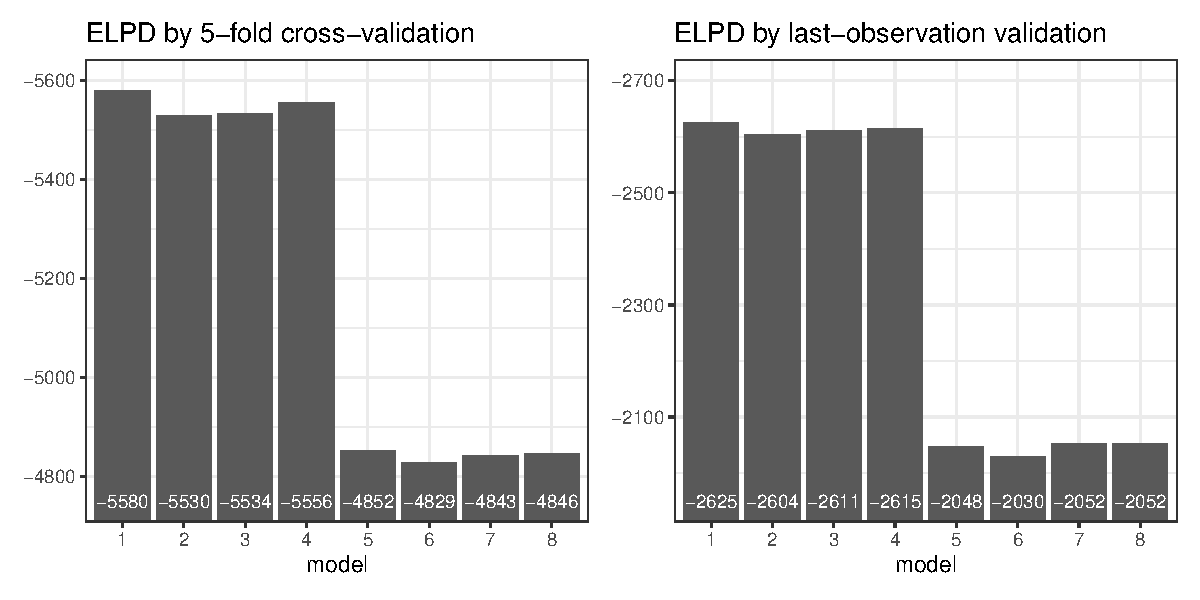
\includegraphics[width=\linewidth]{figures/elpd_plot}
\caption{By these two metrics, the models with transformed MMSE dramatically outperform the models with raw MMSE. Among the transformed models, model 6 does the best, although not by a large margin. Most importantly, it performs no worse, and possibly better, than model 7, which averages the ERC thickness measurements, and model 8, which includes both measurements as outcomes.}
\end{figure}

\pagebreak
\section{Results}

We analyze the joint posterior distribution for model 6. See Tables 2 and 3 for complete results. ANTsSST measures ERC thickness in millimeters. Our transformation of MMSE loss converts it to a roughly standard normal random variable, so the units are now standard deviations, which do not map linearly to scores. In what follows, a parameter is ``significant" if its 90\% Bayesian posterior credible interval does not include 0, and two parameters are ``significantly different" if their intervals do not overlap. 

For the CN and MCI groups, age has a modest but significant association with MMSE: each additional year of age predicts roughly .01 units of MMSE loss. For the MCI group, males have significantly lower (-.133) MMSE loss on average. For all three groups, age has a significant association with ERC thickness: each year of age predicts a difference of -.070, -.062, and -.094, respectively. However, the posterior intervals for the coefficients for CN and MCI overlap, as do those for MCI and AD. For the CN group, males have significantly higher (.289) ERC thickness on average. 

The population means of the MMSE subject-specific intercepts vary significantly across groups, with posterior intervals (-.920, -.791), (.-042, .131), and (.600, .755), for CN, MCI, and AD respectively. The population means of the MMSE subject-specific slopes show the same pattern, with posterior intervals (-.008, .047), (.115, .180), and (.253, .361). Thus, holding age and gender constant, subjects with more advanced disease state perform worse on the MMSE at baseline, and also lose ability more quickly over time. 

The population means of the ERC thickness subject-specific slopes vary significantly across groups, with posterior intervals (7.798, 8.197), (6.884, 7.352), and (5.872, 6.505), for CN, MCI, and AD respectively. The population means of the ERC thickness subject-specific slopes show the same pattern, with posterior intervals (-.059, -.006), (-.133, -.087), and (-.214, -.123). Thus, holding age and gender constant, subjects with more advanced diseased state have less ERC thickness at baseline, and also lose thickness more quickly over time. 

For the MCI and AD groups, MMSE intercept and slope have positive correlations, .497 and .435, that are significantly different from 0 but not from each other. Thus subjects in these groups with less MMSE loss at baseline experience faster decline over time. Also, MMSE intercept and ERC intercept have negative correlations, -.214 and -.461, that are significantly different from 0 but not from each other. Thus subjects with less ERC thickness at baseline have more MMSE loss at baseline. For the MCI group, MMSE slope and ERC slope have significant negative correlation (-.699), meaning that faster MMSE loss correlates with faster ERC loss. For the CN and MCI groups, ERC intercept and ERC slope have positive correlations, .382 and .459, that are significantly different from 0 but not from each other. Thus subjects with more ERC at baseline lose it more slowly. 

\pagebreak
\begin{table}[H]
\centering
\caption{Regression results, model 6}
\begin{tabular}{|l|l|r|r|r|r|}
  \hline
  parameter description & group & mean & sd & q05 & q95 \\ 
  \hline
  age(c) coef MMSE & CN & 0.011 & 0.005 & 0.003 & 0.019 \\ 
  & MCI & 0.009 & 0.004 & 0.001 & 0.016 \\ 
  & AD & -0.001 & 0.004 & -0.008 & 0.006 \\ 
  male coef MMSE & CN & 0.079 & 0.048 & -0.001 & 0.158 \\ 
  & MCI & -0.133 & 0.065 & -0.240 & -0.028 \\ 
  & AD & 0.093 & 0.067 & -0.017 & 0.206 \\ 
  age(c) ERC & CN & -0.070 & 0.017 & -0.099 & -0.042 \\ 
  & MCI & -0.062 & 0.012 & -0.082 & -0.043 \\ 
  & AD & -0.094 & 0.018 & -0.124 & -0.064 \\ 
  male coef ERC & CN & 0.289 & 0.168 & 0.011 & 0.565 \\ 
  & MCI & 0.222 & 0.173 & -0.060 & 0.504 \\ 
  & AD & 0.264 & 0.271 & -0.187 & 0.699 \\ 
  subject intercept mean MMSE & CN & -0.856 & 0.040 & -0.920 & -0.791 \\ 
  & MCI & 0.045 & 0.052 & -0.042 & 0.131 \\ 
  & AD & 0.677 & 0.047 & 0.600 & 0.755 \\ 
  subject slope mean MMSE & CN & 0.019 & 0.017 & -0.008 & 0.047 \\ 
  & MCI & 0.147 & 0.020 & 0.115 & 0.180 \\ 
  & AD & 0.308 & 0.033 & 0.253 & 0.361 \\ 
  subject intercept mean ERC & CN & 7.995 & 0.122 & 7.798 & 8.197 \\ 
  & MCI & 7.117 & 0.141 & 6.884 & 7.352 \\ 
  & AD & 6.192 & 0.192 & 5.872 & 6.505 \\ 
  subject slope mean ERC & CN & -0.032 & 0.016 & -0.059 & -0.006 \\ 
  & MCI & -0.110 & 0.014 & -0.133 & -0.087 \\ 
  & AD & -0.168 & 0.028 & -0.214 & -0.123 \\ 
  subject intercept sd MMSE & CN & 0.239 & 0.032 & 0.188 & 0.291 \\ 
  & MCI & 0.452 & 0.028 & 0.408 & 0.499 \\ 
  & AD & 0.317 & 0.031 & 0.266 & 0.368 \\ 
  subject slope sd MMSE & CN & 0.050 & 0.029 & 0.007 & 0.101 \\ 
  & MCI & 0.205 & 0.022 & 0.170 & 0.242 \\ 
  & AD & 0.266 & 0.034 & 0.211 & 0.323 \\ 
  subject intercept sd ERC & CN & 1.160 & 0.062 & 1.062 & 1.265 \\ 
  & MCI & 1.503 & 0.061 & 1.407 & 1.607 \\ 
  & AD & 1.632 & 0.102 & 1.476 & 1.808 \\ 
  subject slope sd ERC & CN & 0.095 & 0.028 & 0.048 & 0.139 \\ 
  & MCI & 0.078 & 0.021 & 0.043 & 0.113 \\ 
  & AD & 0.057 & 0.042 & 0.004 & 0.137 \\ 
  residual sd MMSE & CN & 0.441 & 0.014 & 0.418 & 0.465 \\ 
  & MCI & 0.408 & 0.011 & 0.391 & 0.426 \\ 
  & AD & 0.273 & 0.015 & 0.250 & 0.299 \\ 
  residual sd ANTsSST & CN & 0.353 & 0.013 & 0.332 & 0.374 \\ 
  & MCI & 0.367 & 0.009 & 0.352 & 0.382 \\ 
  & AD & 0.357 & 0.016 & 0.332 & 0.384 \\
  \hline
\end{tabular}
\end{table}

\pagebreak
\begin{table}[H]
\centering
\caption{Regression results, model 6, subject-specific correlations}
\begin{tabular}{|l|l|r|r|r|r|}
  \hline
  parameter description & group & mean & sd & q05 & q95 \\ 
  \hline
  MMSE intercept / MMSE slope & CN & 0.048 & 0.366 & -0.531 & 0.673 \\ 
   & MCI & 0.497 & 0.134 & 0.276 & 0.716 \\ 
   & AD  & 0.435 & 0.164 & 0.169 & 0.708 \\ 
  MMSE intercept / ERC intercept & CN & 0.136 & 0.122 & -0.069 & 0.335 \\ 
  & MCI & -0.214 & 0.067 & -0.320 & -0.100 \\ 
  & AD & -0.461 & 0.091 & -0.606 & -0.304 \\ 
  MMSE intercept / ERC slope & CN & 0.188 & 0.240 & -0.217 & 0.573 \\ 
  & MCI & -0.124 & 0.207 & -0.476 & 0.206 \\ 
  & AD & -0.252 & 0.385 & -0.802 & 0.474 \\ 
  MMSE slope / ERC intercept & CN & -0.203 & 0.310 & -0.709 & 0.310 \\ 
  & MCI & -0.443 & 0.087 & -0.585 & -0.299 \\ 
  & AD & -0.252 & 0.124 & -0.450 & -0.038 \\ 
  MMSE slope / ERC slope & CN & -0.340 & 0.368 & -0.849 & 0.355 \\ 
  & MCI & -0.699 & 0.165 & -0.915 & -0.405 \\ 
  & AD & -0.094 & 0.396 & -0.720 & 0.593 \\ 
  ERC intercept / ERC slope & CN & 0.382 & 0.197 & 0.077 & 0.730 \\ 
  & MCI & 0.459 & 0.181 & 0.168 & 0.764 \\ 
  & AD & 0.240 & 0.372 & -0.441 & 0.787 \\ 
  MMSE residual / ERC residual & CN & -0.021 & 0.047 & -0.097 & 0.058 \\ 
  & MCI & 0.010 & 0.036 & -0.050 & 0.069 \\ 
  & AD & -0.092 & 0.069 & -0.205 & 0.024 \\ 
   \hline
\end{tabular}
\end{table}

\pagebreak
\section{Discussion}

\subsection{Implications for Alzheimer's research}

\subsection{Implications for imaging}

\subsection{Inferring the conditional distribution}

Suppose that, for a subject in the study, at a future timepoint, we want to infer one outcome given the other. Our model gives us the tools to do that. For example, in our dataset, subject 1 is male, age 84.9 at baseline (mean-centered age is 9.6), with diagnosis CN, and last visit 3 years after baseline. Suppose we measure his MMSE score at 4 years, and we want to estimate his ERC thickness; call it $y^*$. Simplifying the notation somewhat from the full model specification, let $\alpha_{11}, \alpha_{12}$ be the CN group's age and male coefficients for transformed MMSE loss; let $\beta_{11}$ and $\beta_{12}$ be this subject's intercept and slope for transformed MMSE loss; and define $\alpha_{21}, \alpha_{22}, \beta_{21}, \beta_{22}$ similarly for ANTsSST. Let $$\begin{bmatrix} v_{11} & v_{12} \\ v_{21} & v_{22} \\ \end{bmatrix}$$ be the residual covariance for the CN group. For each of the $S$ samples of the posterior vector, take these parameters and compute:

$$\begin{bmatrix} \mu_1 \\ \mu_2 \end{bmatrix}
= \begin{bmatrix}
9.6 \alpha_{11} + \alpha_{12} + \beta_{11} + 4 \beta_{12} \\
9.6 \alpha_{21} + \alpha_{22} + \beta_{21} + 4 \beta_{22} \\
\end{bmatrix}$$
$$\mu^{*} = \mu_2 + v_{21} v_{11}^{-1} (y_1 - \mu_1)$$
$$(\sigma^2)^{*} = v_{22} - v_{21} v_{11}^{-1} v_{12}$$

and then draw a sample from the distribution $N(\mu^*, (\sigma^2)^*)$. The distribution of these $S$ samples is the desired predictive distribution. {\color{teal} [Code this up and plot the distribution].} By a similar technique, by symmetrically swapping the subscripts of $\mu^*$ and $(\sigma^2)^*$, we can infer the ERC thickness from the MMSE score. {\color{teal} [Code this up and plot the distribution].}

Suppose we want to estimate this quantity for a subject not in the study. We need to specify age, gender, diagnosis, and timepoint. Rather than using this subject's intercept and slope, we draw from the population of intercepts and slopes. This will result in a more diffuse estimate for $y^*$. For example, {\color{teal} [Code this up and plot the distribution].}

Finally, suppose we want to explore the association of a covariate on one of the outcomes, holding constant the other covariates \emph{and} the other outcomes. For example, given gender, diagnosis, timepoint, \emph{and} ERC thickness, how does MMSE score ($y^*$) change with baseline age? We cannot specify the functional relationship analytically, but we can get posterior distributions for $y^*$ for a specified sequence of ages. {\color{teal} [Code this up and plot: sequence of violin plots].}

\subsection{(final remarks)}

\pagebreak
\section{Appendix A: Stan code for primary model}

\begin{verbatim}
// GENERAL SCRIPT FOR 8 MODELS

data{

  // number of subjects
  int<lower=1> I; 
  
  // total number of observations, each n is ij
  int<lower=1> N; 
  
  // id of nth observation
  array[N] int<lower=1> id; 
  
  // diagnostic group of subject i (CN = 1, MCI = 2, AD = 3)
  array[I] int<lower=1> group; 
  
  // number of outcomes
  int<lower=1> K; 
  
  // vector of outcomes 
  // (e.g. MMSE_loss, FSLong, ANTsSST) for n = 1:N
  array[N] vector[K] y; 
  
  // 1, t, age_c, male
  array[N] row_vector[4] X; 

}

transformed data {}

parameters{
  
  array[3] vector[2*K] alpha;
  array[3] vector[2*K] mu_beta; 
  array[3] vector<lower=0>[2*K] sigma_beta; 
  array[3] vector<lower=0>[K] sigma_epsilon; 
  array[3] cholesky_factor_corr[2*K] L_Rho_beta; 
  array[3] cholesky_factor_corr[K] L_Rho_epsilon; 
  array[I] vector[2*K] z;

}

transformed parameters{
  
  array[N] vector[K] mu_y; 
  array[I] vector[2*K] beta; 
  array[3] cholesky_factor_cov[2*K] L_Sigma_beta;
  array[3] cholesky_factor_cov[K] L_Sigma_epsilon; 

  for (l in 1:3) {
    // turn sd's and cholesky_corr into cholesky_cov
    L_Sigma_epsilon[l] = 
      diag_pre_multiply(sigma_epsilon[l], L_Rho_epsilon[l]);
    L_Sigma_beta[l] = 
      diag_pre_multiply(sigma_beta[l], L_Rho_beta[l]);    
  }
  
  for (i in 1:I) {
    // equivalent to beta[i] ~ multi_normal(mu_beta[group[i]], 
    //                                      Sigma_beta[group[i]])
    beta[i] = mu_beta[group[i]] + L_Sigma_beta[group[i]] * z[i];
  }

  if (K == 2) {
    for (n in 1:N) {
      mu_y[n] = [ X[n] * append_row(beta[id[n]][1:2], 
                                    alpha[group[id[n]]][1:2]),
                  X[n] * append_row(beta[id[n]][3:4], 
                                    alpha[group[id[n]]][3:4])]';
    }
  }

  if (K == 3) {
    for (n in 1:N) {
      mu_y[n] = [ X[n] * append_row(beta[id[n]][1:2], 
                                    alpha[group[id[n]]][1:2]),
                  X[n] * append_row(beta[id[n]][3:4], 
                                    alpha[group[id[n]]][3:4]),
                  X[n] * append_row(beta[id[n]][5:6], 
                                    alpha[group[id[n]]][5:6]) ]';
    }
  }
  
}

model{

  // likelihood
  for (n in 1:N) {
    y[n] ~ multi_normal_cholesky(mu_y[n], 
                                 L_Sigma_epsilon[group[id[n]]]);
  }

  // priors
  for (l in 1:3) {
    
    alpha[l] ~ normal(0, 2); 
    mu_beta[l][1] ~ normal(0, 2); // MMSE intercept mean
    mu_beta[l][2] ~ normal(0, 2); // MMSE slope mean
    sigma_beta[l][1] ~ exponential(1); // MMSE intercept sd
    sigma_beta[l][2] ~ exponential(1); // MMSE slope sd

    mu_beta[l][3] ~ normal(7, 3); // y2 intercept mean
    mu_beta[l][4] ~ normal(0, 1); // y2 slope mean
    sigma_beta[l][3] ~ exponential(1); // y2 intercept sd
    sigma_beta[l][4] ~ exponential(5); // y2 slope sd
    
    if(K == 3){
      mu_beta[l][3] ~ normal(7, 3); // y3 intercept mean
      mu_beta[l][4] ~ normal(0,1); // y3 slope mean
      sigma_beta[l][3] ~ exponential(1); // y3 intercept sd
      sigma_beta[l][4] ~ exponential(5); // y3 slope sd  
    }
    
    L_Rho_beta[l] ~ lkj_corr_cholesky(1);
    sigma_epsilon[l] ~ exponential(1);
    L_Rho_epsilon[l] ~ lkj_corr_cholesky(1);
    
  }
  
  // random effects distribution
  for(i in 1:I){
    z[i] ~ std_normal();
  }
  
}

generated quantities {

  vector[N] log_lik;
  array[3] matrix[2*K,2*K] Rho_beta;
  array[3] matrix[K,K] Rho_epsilon;
  array[3] matrix[2*K,2*K] Sigma_beta;
  array[3] matrix[K,K] Sigma_epsilon;

  for (n in 1:N) {
    log_lik[n] = multi_normal_cholesky_lpdf(
      y[n] | mu_y[n], 
      L_Sigma_epsilon[group[id[n]]]);
  }

  for (l in 1:3) {
    Rho_beta[l] = L_Rho_beta[l] * L_Rho_beta[l]';
    Rho_epsilon[l] = L_Rho_epsilon[l] * L_Rho_epsilon[l]';  
    Sigma_beta[l] = L_Sigma_beta[l] * L_Sigma_beta[l]';
    Sigma_epsilon[l] = L_Sigma_epsilon[l] * L_Sigma_epsilon[l]';
  }

}
\end{verbatim}

\pagebreak
\bibliographystyle{sysbio}
\bibliography{refs}

\end{document}

Clearly the transformed model does better
Only disadvantage is difficulty of interpretation
Here's a table

Among transformed models:
We run CVs 3 times, to see if the small differences are "significant"

What do we find about age? gender? group comparison? distr of intercepts and slopes? cov of intercepts and slopes?

In 3v model, how much of a difference in these parameters? 

Demo: use conditional MVN formula to explore relationships between outcomes, in example model

Effect of transformation: Comparing models with transformation to the corresponding models without, we see LEPD increase by about 700. Since there are 2449 observations in the data, and exp(700/2449)=1.33, the transformed model has a typical likelihood 1.33 times higher per observation. (How else to interpret this? Likelihood ratio? Bayes factor?)
